\documentclass[10pt,a4paper]{article}

\usepackage[utf8]{inputenc}
\usepackage[T1]{fontenc}
\usepackage[margin=2.5cm]{geometry}
\usepackage{graphicx}
\usepackage{booktabs}
\usepackage{amsmath}
\usepackage{amssymb}
\usepackage{hyperref}
\usepackage{caption}
\usepackage{subcaption}
\usepackage{xcolor}
\usepackage{float}
\usepackage{multirow}
\usepackage{array}

\hypersetup{
    colorlinks=true,
    linkcolor=black,
    citecolor=black,
    urlcolor=blue,
}

\graphicspath{{plots/}}

\title{\textbf{Project 22: Movie Revenue Prediction}\\
\large A Comparative Study of Six Regression Algorithms on TMDB Box-Office Data}
\author{Engin S.\ Demirkan \and Franziska Axmann}
\date{June 2026}

\begin{document}
\maketitle

\begin{abstract}
We study the problem of predicting global box-office revenue for individual films from
metadata available at release time. Starting from the official TMDB Box Office
Prediction dataset (3{,}000 films), we engineer 49 numerical, binary, and categorical
features capturing budget, popularity, temporal context, cast composition, genre
membership, language, and metadata richness. Recognising that the raw revenue
spans nine orders of magnitude, we adopt a $\log(1{+}y)$ target transformation and
compare six regression algorithms — Linear Regression, Ridge Regression, Random
Forest, XGBoost, LightGBM, and CatBoost — under an identical preprocessing pipeline
and 5-fold cross-validation. The strongest model, CatBoost, attains a
cross-validated RMSLE of $1.584{\pm}0.029$, while Random Forest reaches a hold-out
$R^{2}$ of $0.709$ and a Median Absolute Percentage Error of $66.5\%$. An ablation
study isolates the contribution of each feature group and shows that budget
(\(+0.133\) RMSLE if removed), popularity/runtime (\(+0.110\)), and temporal
signals (\(+0.081\)) are the three dominant drivers; genre flags contribute a
modest but real $+0.029$. All experiments use a fixed random seed; the complete
pipeline is reproducible from a single command.
\end{abstract}

\section{Introduction}

Predicting the box-office revenue of a film from its pre-release metadata is a
classic supervised-learning problem with a heavy-tailed target distribution,
mixed feature types, and a moderate sample size. It is the subject of a Kaggle
competition based on data from The Movie Database (TMDB), which provides the
canonical benchmark used in this work.

Our preliminary submission for this project used a single XGBoost model with six
input features, achieving an $R^{2}$ of $0.6352$. Reviewer feedback during the
midterm consultation highlighted three concerns: (i) the absence of any
comparative analysis across model families, (ii) a Mean Absolute Percentage Error
(MAPE) value of $2{,}096\%$ that was not explained, and (iii) the use of only a
small subset of the available features.

This final report addresses each concern directly. We retrain the system from
scratch with a richer feature space, compare six regression algorithms drawn
from the linear and tree-based families, justify the choice of evaluation
metrics for a heavy-tailed target, and perform a feature-group ablation study to
attribute performance to its sources.

\section{Dataset}

The TMDB Box Office Prediction dataset contains \(3{,}000\) labelled films with
\(23\) columns each: budget, popularity, runtime, original language, release
date, and several JSON-encoded list fields (genres, production companies and
countries, spoken languages, keywords, cast, and crew). Films flagged with a
revenue placeholder of \(\le \$1{,}000\) are Kaggle artefacts (1$ or 5$ stand-ins for
unknown values) and were removed, leaving \(2{,}943\) usable films. We use a
single \(80/20\) train/test split for the headline metrics and additionally
report \(5\)-fold cross-validation on the full preprocessed set for stability.

The revenue distribution is extremely right-skewed
(Figure~\ref{fig:revenue_dist}): a small number of blockbusters earn nearly
\$1.5 billion, while the median release earns just under \$17M. The log-transformed
target is approximately Gaussian, which makes the squared-error loss used by all
six models a much better fit and justifies our choice of a $\log(1{+}y)$ target.

\begin{figure}[H]
\centering
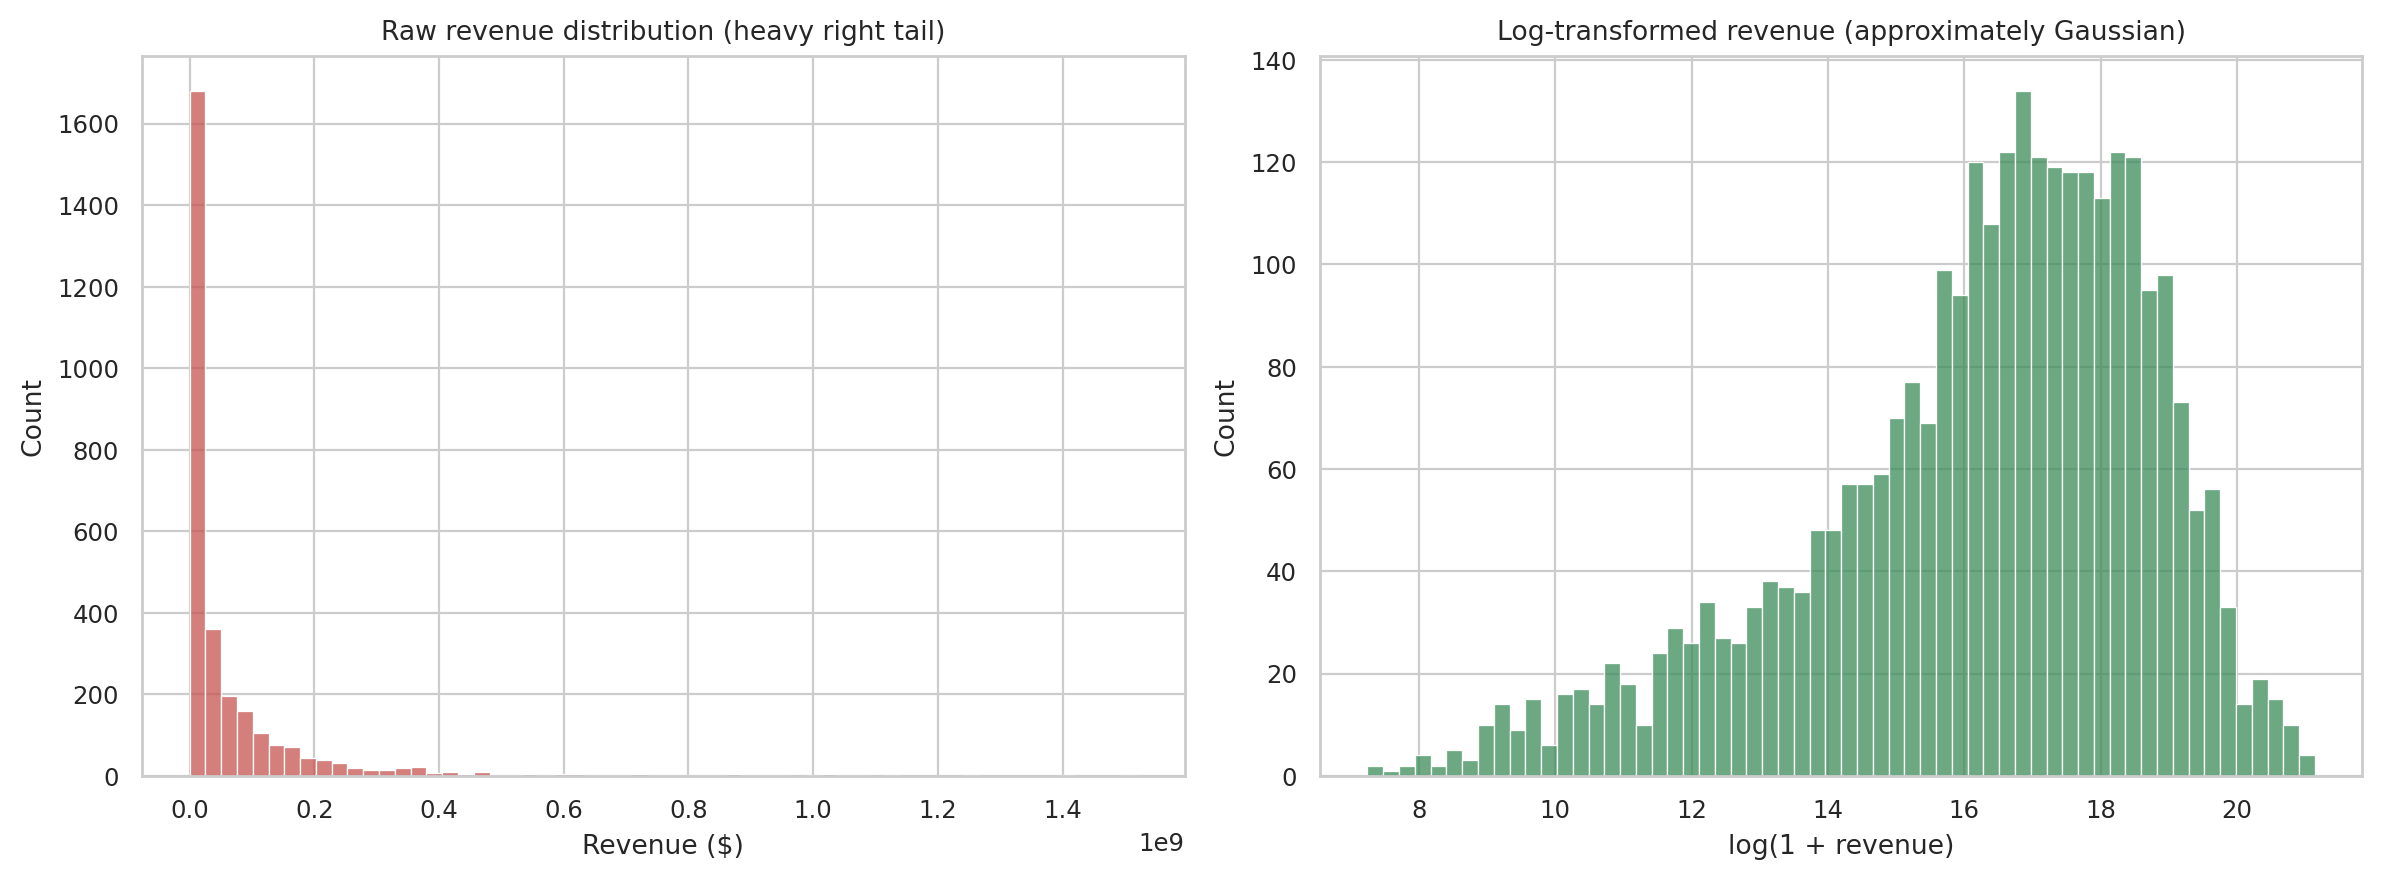
\includegraphics[width=0.95\linewidth]{01_revenue_distribution}
\caption{Raw revenue (left) versus log-transformed revenue (right). The raw
distribution is extreme-tailed; the log target is approximately symmetric.}
\label{fig:revenue_dist}
\end{figure}

\subsection{Feature Engineering}

Parsing each JSON-encoded list column and combining the result with the simple
columns yields \(49\) features organised into eight semantic groups
(Table~\ref{tab:feature_groups}). The dominant design choices are:
\begin{itemize}
    \item \textbf{Budget transforms.} \(\log(1{+}\text{budget})\) compresses the
        feature scale; a binary \texttt{budget\_missing} flag is added because
        roughly 27\% of films have a placeholder value of \(0\), and the
        boundary between $\$0$ and a low-budget independent film should be
        accessible to the trees.
    \item \textbf{Temporal signals.} Release year, month, quarter, day-of-week,
        and decade, plus boolean flags for summer (Jun–Aug) and holiday (Nov–Dec)
        release windows.
    \item \textbf{Metadata presence flags.} Whether the film has a homepage, a
        tagline, a collection (i.e.\ belongs to a franchise), and whether the
        translated title differs from the original.
    \item \textbf{List counts.} Number of cast members, crew members, genres,
        production companies, production countries, spoken languages, and
        keywords. Gender composition of the cast is split into three counts.
    \item \textbf{Genre multi-label flags.} Binary indicators for the 15 most
        frequent genres.
\end{itemize}

\begin{table}[H]
\centering
\small
\begin{tabular}{lcl}
\toprule
Feature group & \# features & Examples \\
\midrule
Budget         & 4  & \texttt{budget\_log}, \texttt{budget\_missing}, \texttt{budget\_per\_minute} \\
Popularity / runtime  & 2  & \texttt{popularity}, \texttt{runtime} \\
Temporal       & 7  & \texttt{release\_year}, \texttt{release\_month}, \texttt{is\_summer\_release} \\
Counts         & 10 & \texttt{n\_cast}, \texttt{n\_crew}, \texttt{cast\_n\_male} \\
Presence flags & 6  & \texttt{has\_collection}, \texttt{has\_homepage}, \texttt{is\_english} \\
Text lengths   & 4  & \texttt{overview\_len}, \texttt{title\_len}, \texttt{tagline\_len} \\
Genre flags    & 15 & \texttt{genre\_drama}, \texttt{genre\_action}, \texttt{genre\_horror} \\
Language       & 1  & \texttt{lang\_grouped} (top-10 + ``other'') \\
\midrule
Total          & 49 & \\
\bottomrule
\end{tabular}
\caption{The 49 engineered features, organised by semantic group. Each group is
used as a unit in the ablation study of Section~\ref{sec:ablation}.}
\label{tab:feature_groups}
\end{table}

\section{Methods}

\subsection{Models Compared}

We evaluate six regression algorithms drawn from two families.

\textbf{Linear family.}
\textit{Linear Regression} fits a closed-form least-squares hyperplane. It serves
as a low-capacity baseline. \textit{Ridge Regression} adds an
$L_{2}$ penalty $\alpha\|\beta\|_{2}^{2}$ on the coefficients, which can stabilise
the fit when features are correlated; we use $\alpha=1$.

\textbf{Tree-based ensembles.}
\textit{Random Forest} fits a large number of de-correlated decision trees on
bootstrap samples and averages their predictions. We use 400 trees,
\texttt{max\_depth=12}, and \texttt{min\_samples\_leaf=2}.
\textit{XGBoost}~\cite{xgboost} builds trees sequentially with second-order
gradient information and an explicit complexity penalty; we use 600 estimators,
learning rate $0.05$, \texttt{max\_depth=6}, and column/row subsampling at $0.8$.
\textit{LightGBM}~\cite{lightgbm} uses histogram-based splits and leaf-wise growth
for speed; we use 800 estimators with 31 leaves per tree, same learning rate
and subsampling. \textit{CatBoost}~\cite{catboost} uses ordered boosting and
symmetric (oblivious) trees that are robust to overfitting and require minimal
tuning; we use 800 iterations, depth 6, and $\ell_{2}$ leaf regularisation 3.

All hyperparameters were fixed before evaluation; we did not perform additional
grid search, both for reproducibility and because the goal of the project is a
fair comparison rather than absolute tuning.

\subsection{Preprocessing Pipeline}

For every model we apply the same preprocessing pipeline, encapsulated as a
single \texttt{ColumnTransformer}:
\begin{itemize}
    \item Numerical features: median imputation of missing values; standard
          scaling (mean 0, unit variance) for the linear models only, since
          tree-based models are scale-invariant.
    \item The single categorical feature (\texttt{lang\_grouped}): most-frequent
          imputation followed by one-hot encoding with
          \texttt{handle\_unknown=ignore} so that languages unseen in a fold do
          not crash inference.
\end{itemize}
The full pipeline is a scikit-learn \texttt{Pipeline} object so that the
preprocessor is fitted only on each fold's training data, which prevents
data leakage in cross-validation.

\subsection{Target Transformation and Evaluation Metrics}

The training target is $z = \log(1{+}y)$, where $y$ is the revenue in dollars.
At inference time we clip predictions in log space to the training range
$[z_{\min}, z_{\max}]$ before applying \texttt{expm1} — a standard no-extrapolation
guard that primarily affects the linear models, which can otherwise produce
unrealistically large predictions.

We report the following metrics on dollar-space predictions:

\begin{align}
\mathrm{RMSE}  &= \sqrt{\tfrac{1}{n}\sum_{i=1}^{n}(y_i - \hat y_i)^{2}} \\
\mathrm{R}^{2} &= 1 - \frac{\sum_{i}(y_i - \hat y_i)^{2}}{\sum_{i}(y_i - \bar y)^{2}} \\
\mathrm{RMSLE} &= \sqrt{\tfrac{1}{n}\sum_{i=1}^{n}\bigl(\log(1{+}y_i) - \log(1{+}\hat y_i)\bigr)^{2}} \\
\mathrm{MAPE}  &= \tfrac{100}{n}\sum_{i=1}^{n}\left|\frac{y_i - \hat y_i}{y_i}\right|, \quad
\mathrm{MedAPE}  = 100 \cdot \mathrm{median}_{i}\left|\frac{y_i - \hat y_i}{y_i}\right|
\end{align}

\paragraph{Why MAPE alone is unreliable.}
MAPE is the metric requested for this project but is well known to be unstable
on heavy-tailed positive targets. A single film whose true revenue is, say,
$\$50{,}000$ but whose prediction is $\$1$M contributes a $1{,}900\%$ error to the
average, which then dominates the metric regardless of how well the other 599
test films are predicted. We address this in two complementary ways. First, we
filter out the placeholder revenues $\le \$1{,}000$ that are pure noise. Second,
we additionally report the \emph{median} absolute percentage error
(\textbf{MedAPE}), which is the standard robust alternative and represents the
typical relative error of a film rather than the mean contaminated by outliers.
Throughout the discussion we treat \textbf{RMSLE} as the primary metric — it is
also the official Kaggle competition metric for this dataset — and use MedAPE as
the human-readable companion.

\section{Results}

Table~\ref{tab:results} reports every metric for every model. CatBoost wins the
cross-validation leaderboard on the primary metric (CV-RMSLE \(=1.584\pm0.029\)),
while Random Forest narrowly wins the hold-out $R^{2}$ at \(0.709\); the two
results are consistent up to the noise level of a single $80/20$ split. All four
tree-based ensembles outperform the linear baselines by a wide margin on every
metric (Figure~\ref{fig:rmsle_bar}), confirming that the input-to-revenue mapping
is strongly non-linear.

\begin{table}[H]
\centering
\small
\setlength{\tabcolsep}{4pt}
\begin{tabular}{lrrrrrr}
\toprule
Model & RMSE (\$M) & $R^{2}$ & RMSLE & MedAPE & MAPE & CV-RMSLE \\
\midrule
Linear Regression & 128.1 & 0.199 & 1.669 & 69.8\%  & 966\%  & $1.777 \pm 0.066$ \\
Ridge Regression  & 129.5 & 0.182 & 1.670 & 69.4\%  & 968\%  & $1.776 \pm 0.065$ \\
Random Forest     &  77.2 & \textbf{0.709} & 1.577 & 66.5\%  & 574\%  & $1.614 \pm 0.032$ \\
XGBoost           &  77.3 & 0.709 & 1.569 & 65.5\%  & 612\%  & $1.614 \pm 0.044$ \\
LightGBM          &  83.9 & 0.656 & 1.582 & 65.3\%  & \textbf{547\%}  & $1.642 \pm 0.048$ \\
\textbf{CatBoost} &  82.3 & 0.670 & \textbf{1.539} & \textbf{65.4\%}  & 561\%  & $\mathbf{1.584 \pm 0.029}$ \\
\bottomrule
\end{tabular}
\caption{Hold-out test metrics ($80/20$ split, $n=589$) plus $5$-fold
cross-validation RMSLE on the full \(2{,}943\)-film set. Best per metric in bold.
RMSE is reported in millions of dollars for readability.}
\label{tab:results}
\end{table}

\begin{figure}[H]
\centering
\begin{subfigure}{0.48\linewidth}
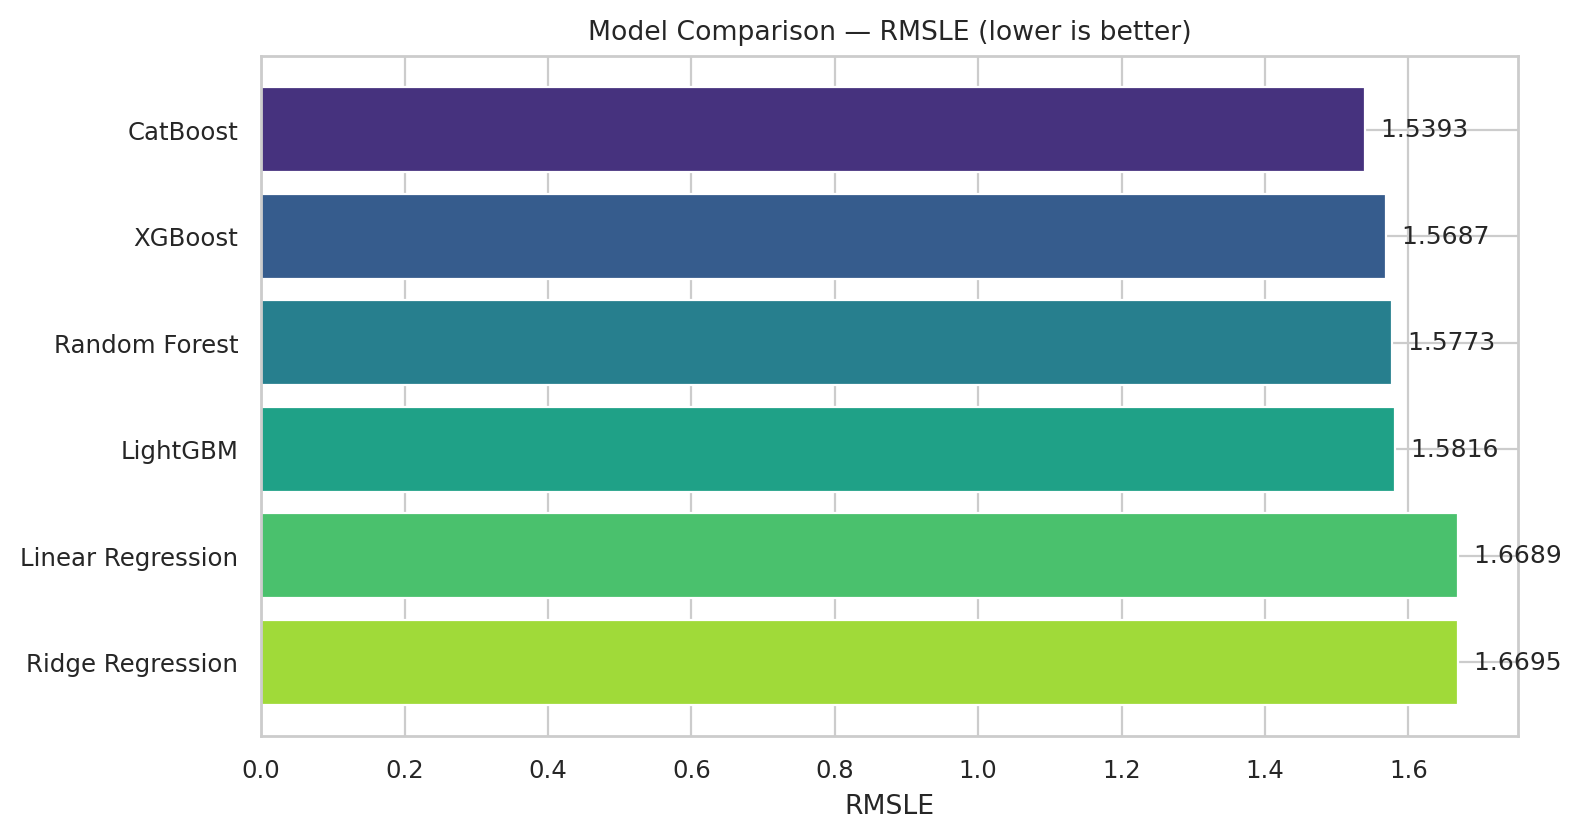
\includegraphics[width=\linewidth]{03_rmsle_comparison}
\caption{RMSLE — lower is better.}
\end{subfigure}
\hfill
\begin{subfigure}{0.48\linewidth}
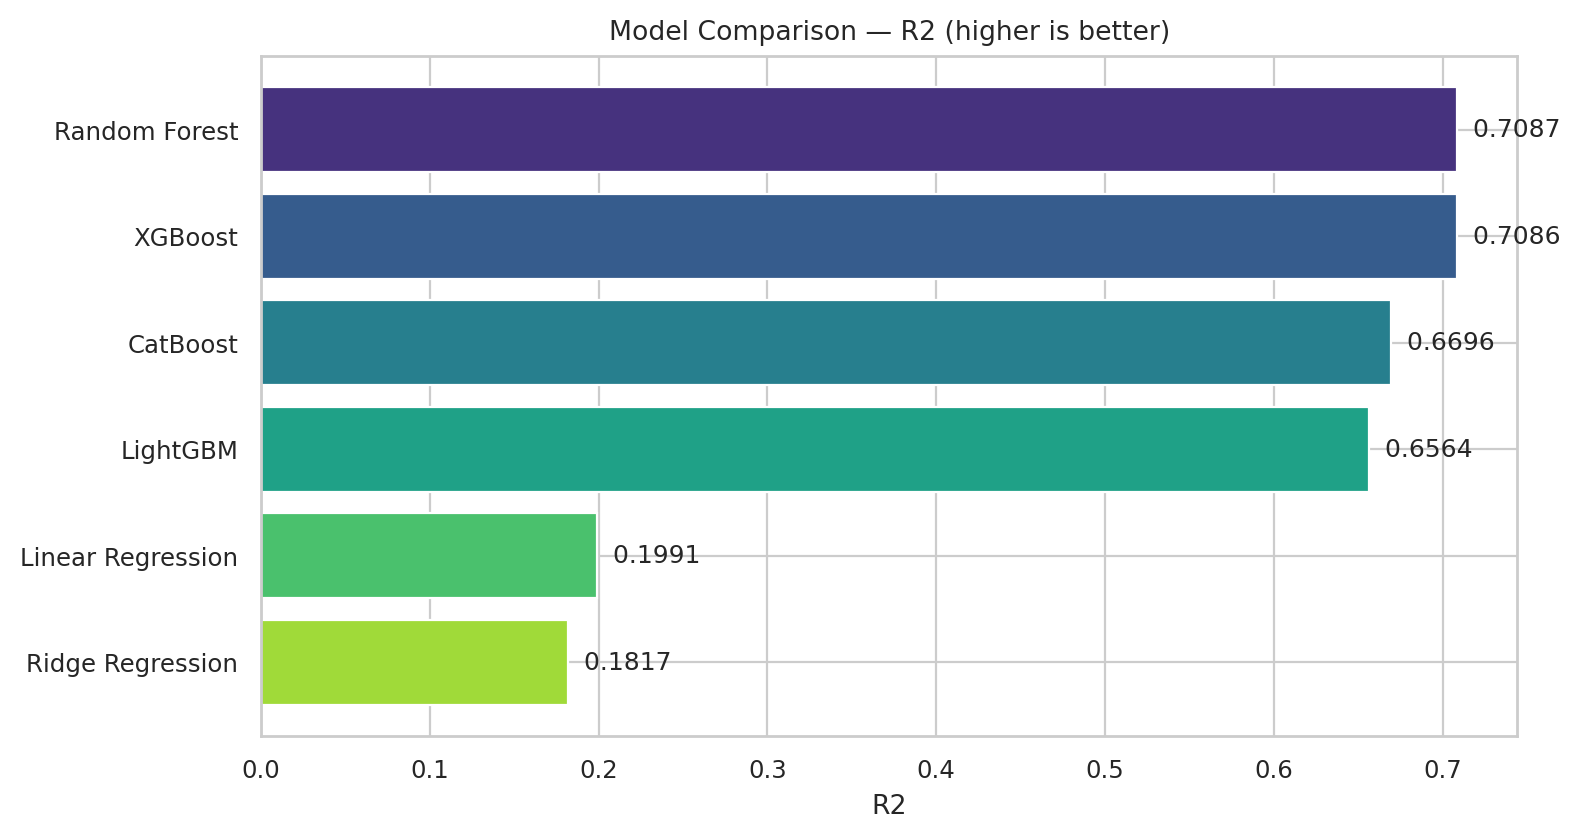
\includegraphics[width=\linewidth]{04_r2_comparison}
\caption{$R^{2}$ on the hold-out test set.}
\end{subfigure}
\caption{Two views of the model comparison. Tree-based ensembles cluster around
RMSLE $\approx 1.55$--$1.58$, well below the linear baselines at $\approx 1.67$.}
\label{fig:rmsle_bar}
\end{figure}

\begin{figure}[H]
\centering
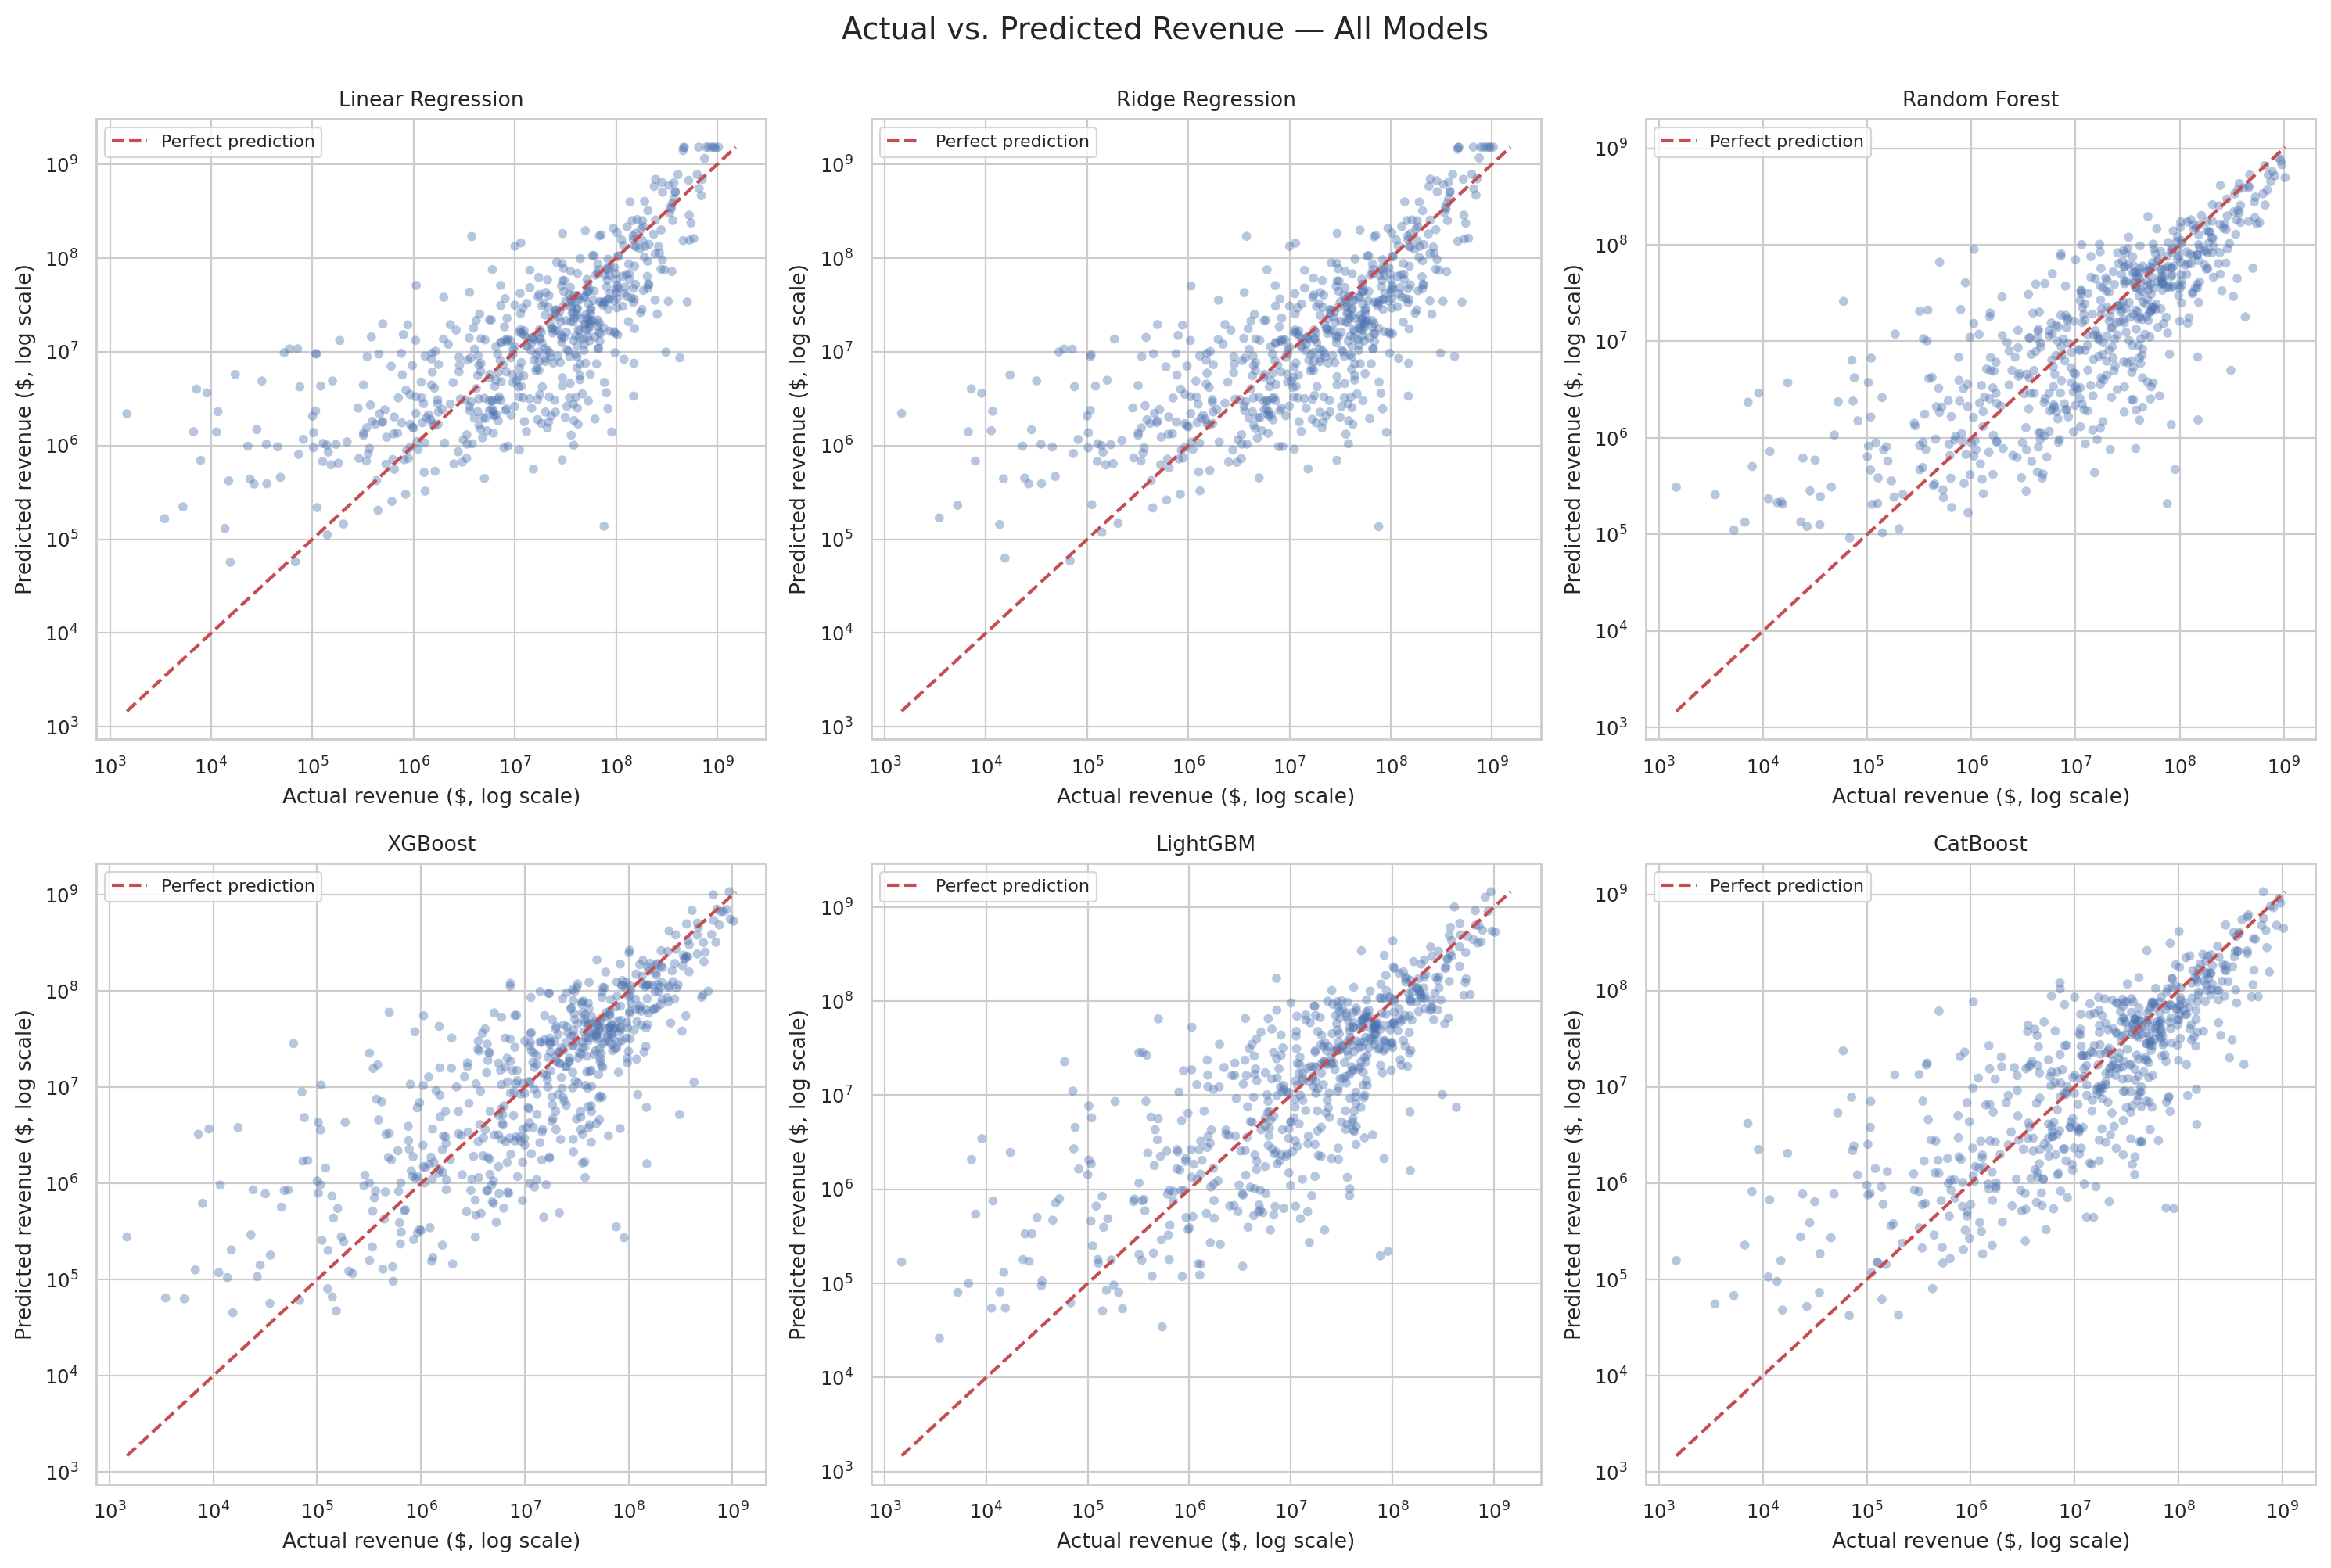
\includegraphics[width=0.98\linewidth]{02_actual_vs_predicted_grid}
\caption{Actual vs predicted revenue, both axes on log scale, one panel per
model. Tighter clouds along the diagonal indicate better fit. The linear models
(top row) show visible heteroscedasticity and a systematic over-prediction for
small-revenue films; the tree ensembles (bottom row) recover the relationship
across the full nine-order-of-magnitude range.}
\label{fig:scatter_grid}
\end{figure}

\subsection{Residual Analysis}

Figure~\ref{fig:residuals} shows that CatBoost residuals in log space are
approximately Gaussian with mean near zero and a mild negative skew at the
low-revenue end. This skew is the source of most of the remaining MAPE: when
the model predicts $\$2$M for a film whose actual revenue is $\$50$k, the
absolute residual in log space is moderate ($\log 40 \approx 3.7$) but the
percentage error is $3{,}900\%$. The RMSLE and MedAPE columns of
Table~\ref{tab:results} are not affected by these outliers, which is why we use
them as the headline metrics.

\begin{figure}[H]
\centering
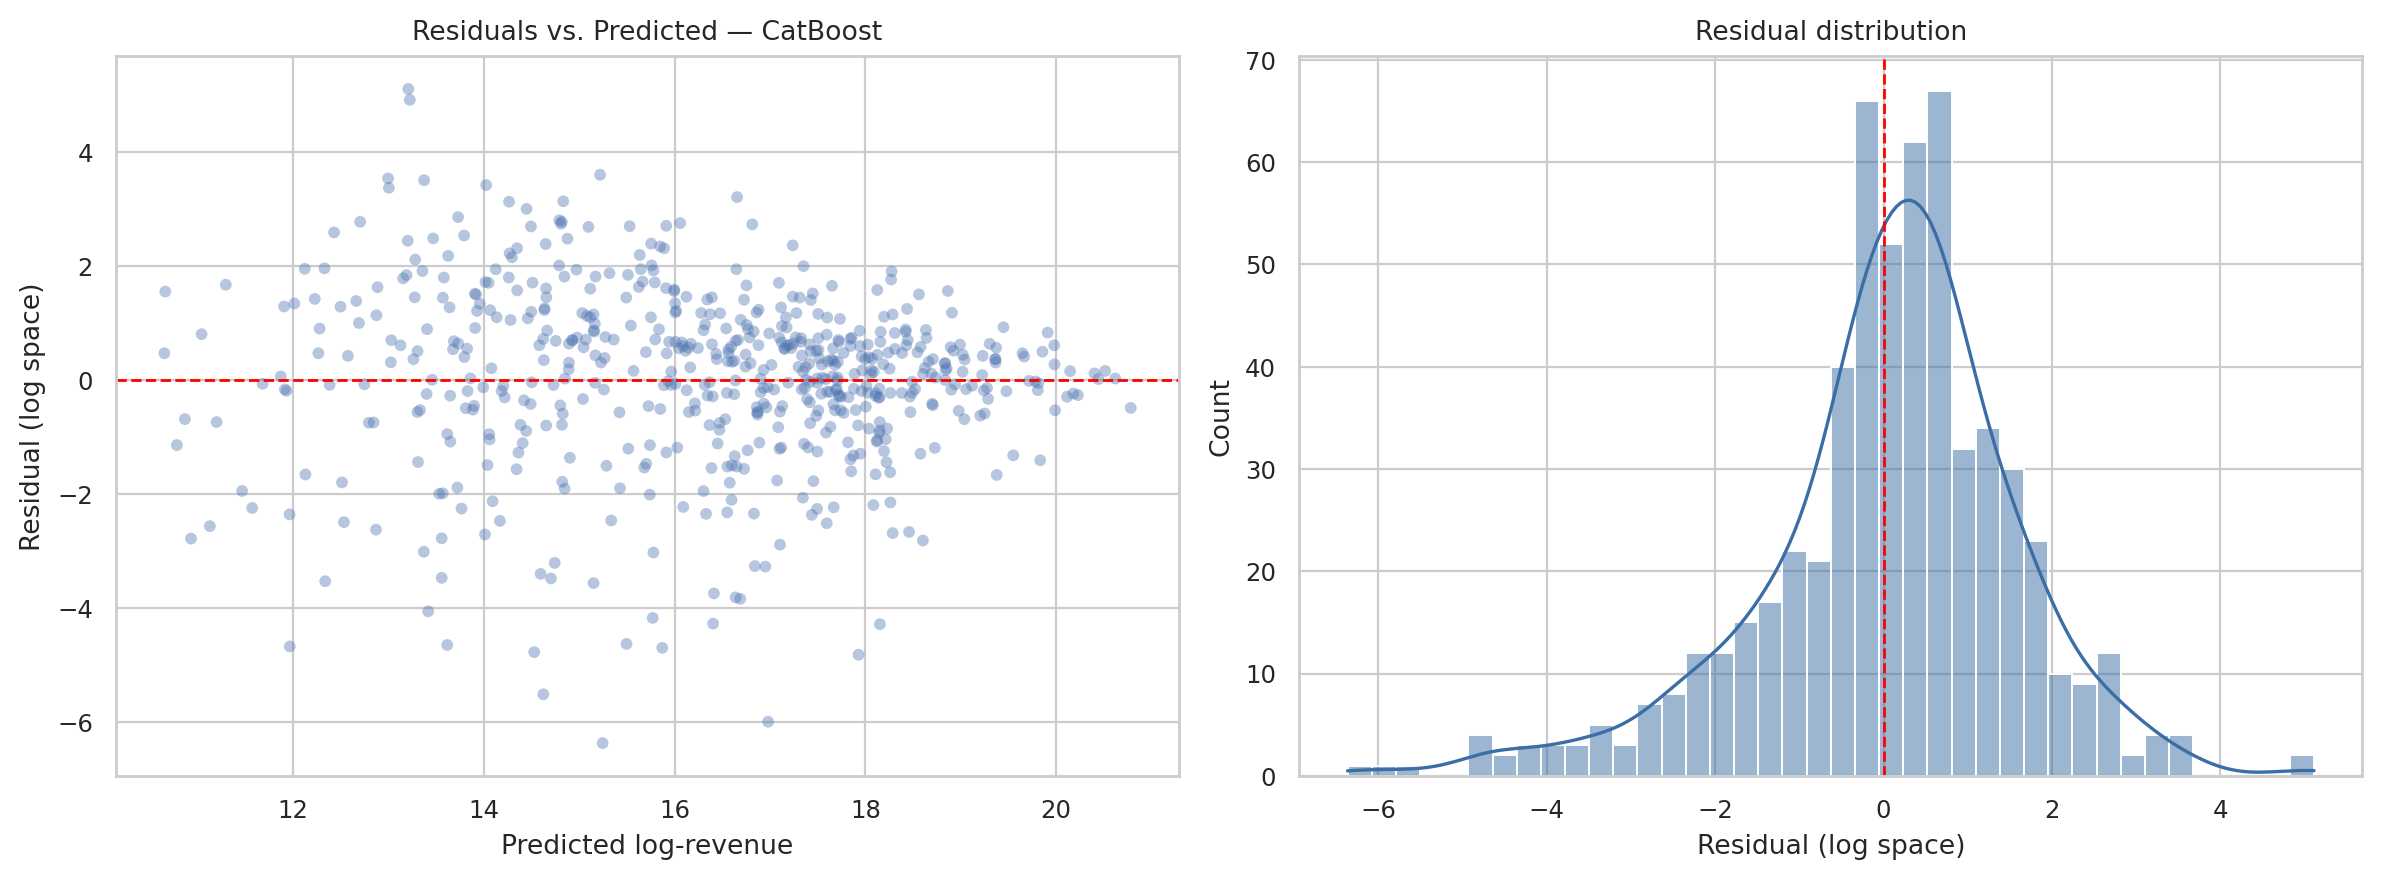
\includegraphics[width=0.95\linewidth]{06_residuals_best}
\caption{CatBoost residuals in log space. Left: residuals vs predicted
log-revenue; right: residual distribution. The residuals are centred near zero
and approximately Gaussian, with a heavier left tail corresponding to films
whose revenue the model overestimates.}
\label{fig:residuals}
\end{figure}

\subsection{Feature Importance}

Figure~\ref{fig:importance} ranks the top 20 features by CatBoost's internal
importance scores. Five engineered numerical features dominate: \texttt{popularity},
\texttt{budget\_per\_minute}, \texttt{budget\_log}, \texttt{release\_year}, and
\texttt{runtime}. The high rank of the engineered \texttt{budget\_per\_minute}
(production density) and \texttt{budget\_log} features above the raw
\texttt{budget} confirms that the log transform is informative even as an input,
not just as a target.

\begin{figure}[H]
\centering
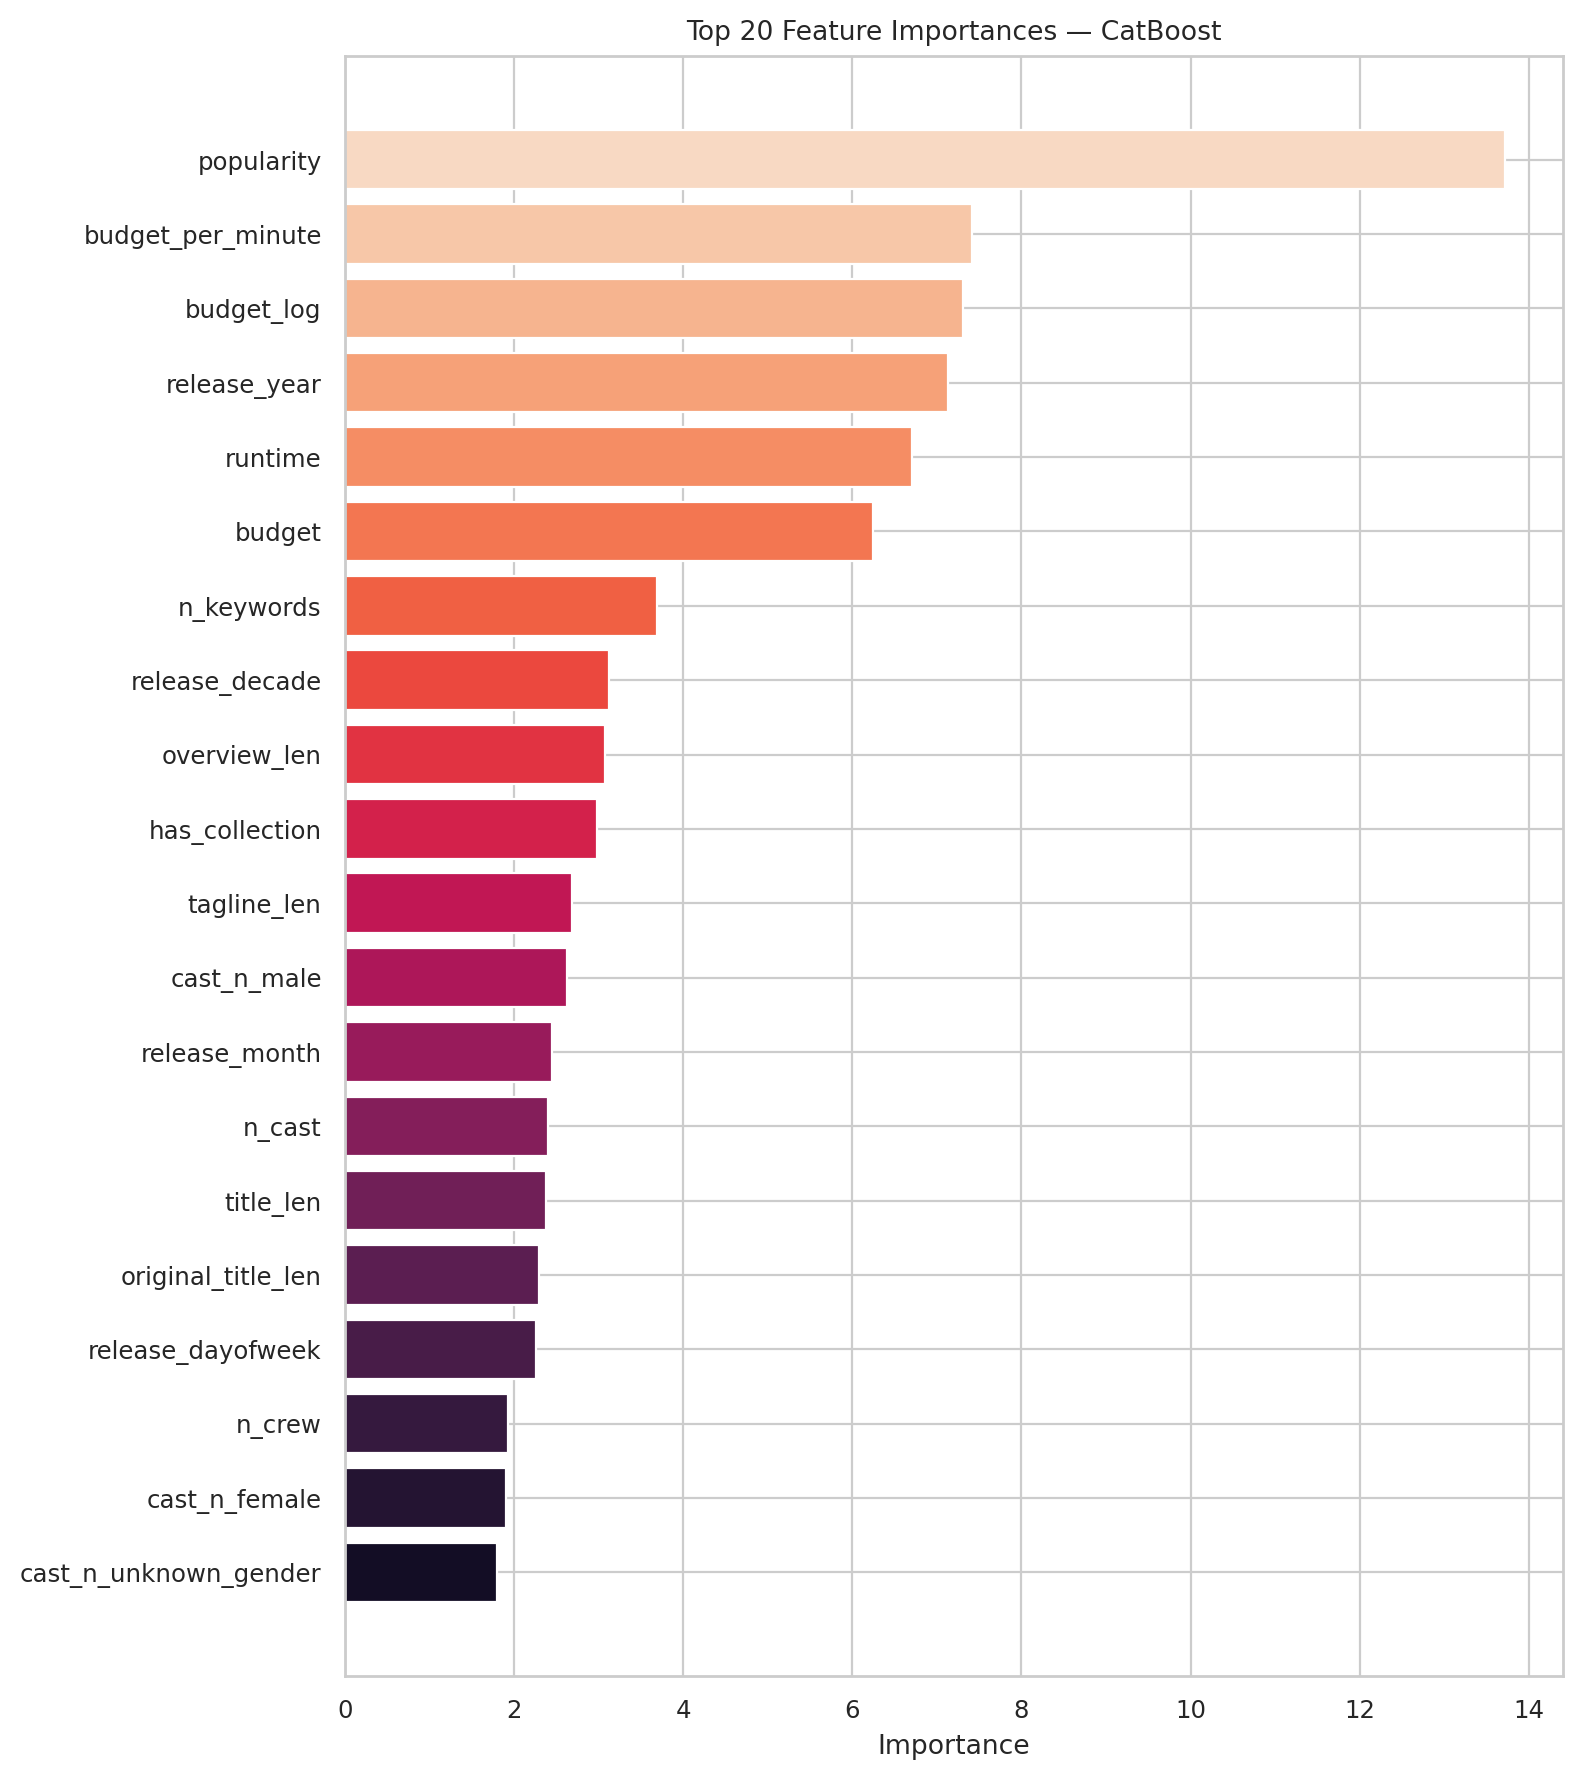
\includegraphics[width=0.75\linewidth]{07_feature_importance_best}
\caption{Top 20 features by CatBoost importance. The five most important
features are all continuous; engineered budget and temporal features outrank
the raw budget column.}
\label{fig:importance}
\end{figure}

\subsection{Ablation Study}
\label{sec:ablation}

To attribute performance to feature groups rather than individual features, we
re-ran CatBoost 5-fold cross-validation with each of the eight semantic groups
in Table~\ref{tab:feature_groups} \emph{removed} in turn. The reported quantity
is $\Delta\mathrm{RMSLE} = \mathrm{RMSLE}_{\text{ablated}} - \mathrm{RMSLE}_{\text{baseline}}$:
larger values mean the group is more important. Results are in
Figure~\ref{fig:ablation} and Table~\ref{tab:ablation}.

\begin{table}[H]
\centering
\small
\begin{tabular}{lrr}
\toprule
Group removed       & CV-RMSLE & $\Delta$ vs. baseline \\
\midrule
\emph{Baseline} (all features) & 1.584 & --- \\
Budget              & 1.717 & $+0.133$ \\
Popularity/runtime  & 1.693 & $+0.110$ \\
Temporal            & 1.665 & $+0.081$ \\
Genre flags         & 1.613 & $+0.029$ \\
Presence flags      & 1.593 & $+0.009$ \\
Language            & 1.591 & $+0.007$ \\
Counts              & 1.585 & $+0.001$ \\
Text lengths        & 1.568 & $-0.016$ \\
\bottomrule
\end{tabular}
\caption{Ablation: 5-fold CV-RMSLE when one feature group is dropped. The
last row shows that text-length features marginally hurt CV performance.}
\label{tab:ablation}
\end{table}

\begin{figure}[H]
\centering
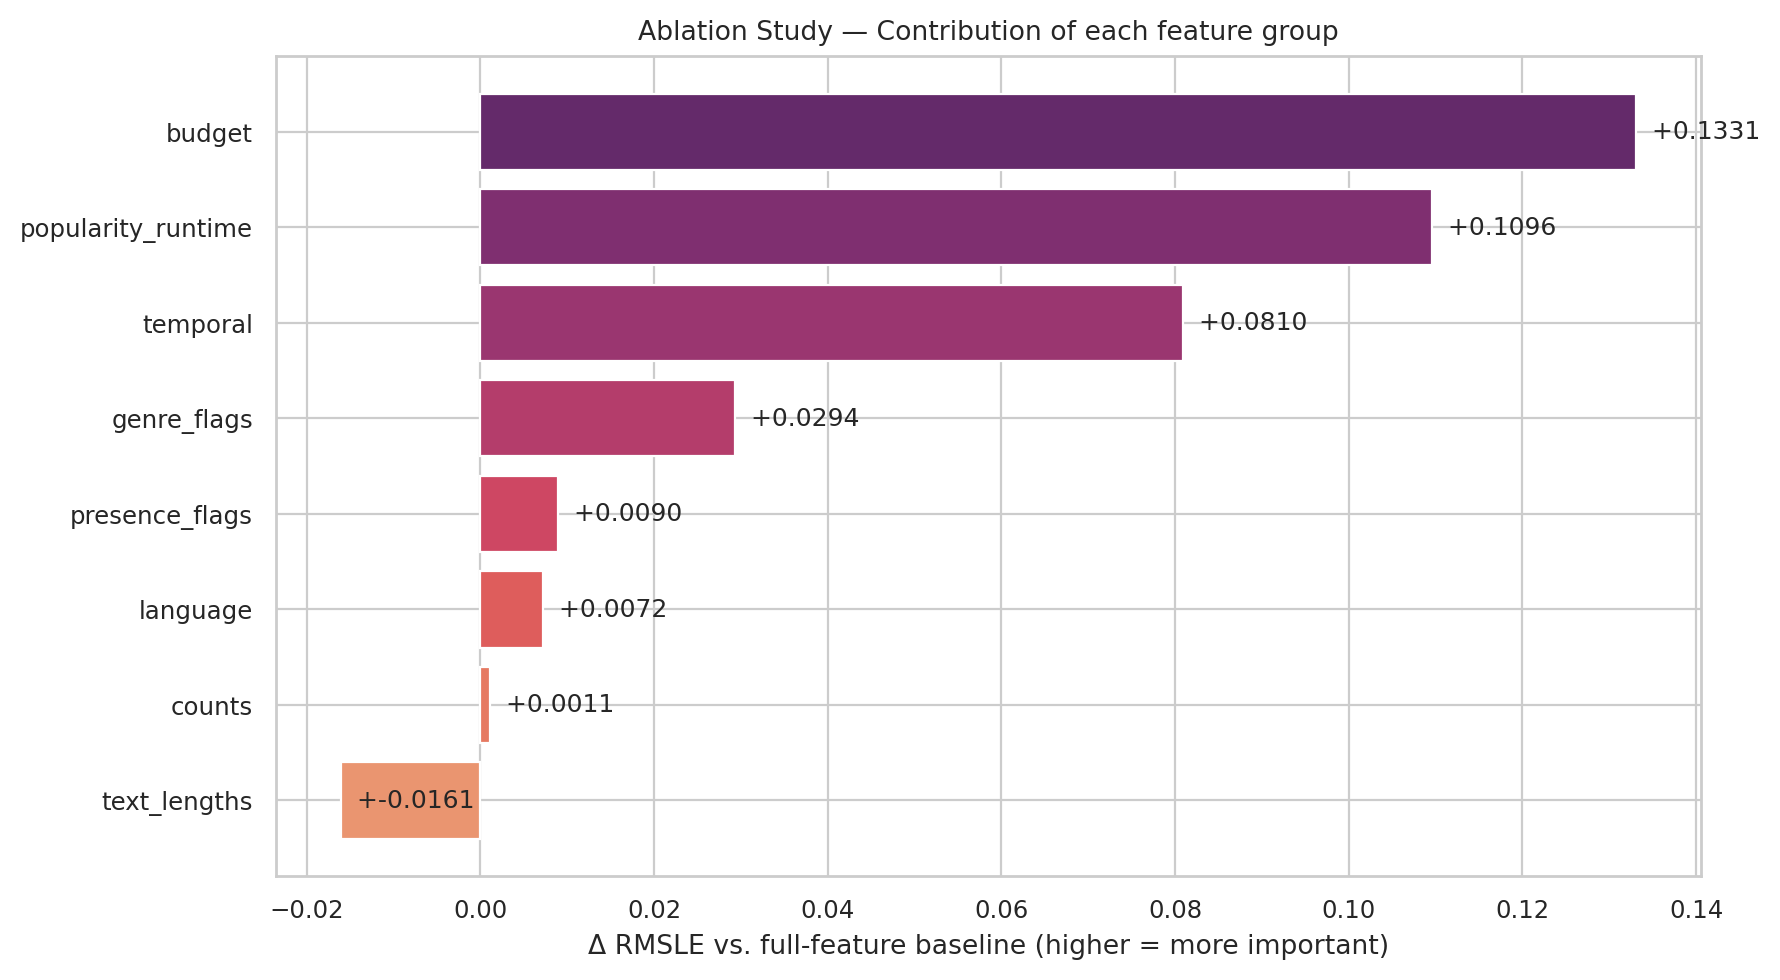
\includegraphics[width=0.85\linewidth]{08_ablation_study}
\caption{Ablation study: change in 5-fold CV-RMSLE relative to the
full-feature baseline when each feature group is removed. Bars to the right are
groups whose removal hurts performance; the single bar to the left
(\texttt{text\_lengths}) is a group whose removal actually \emph{improves}
performance, suggesting it acts as noise.}
\label{fig:ablation}
\end{figure}

The three dominant groups — \emph{budget}, \emph{popularity/runtime}, and
\emph{temporal} — together account for $+0.32$ RMSLE if jointly removed, which
is more than the gap between the strongest tree model and the weakest linear
model ($1.670 - 1.539 = 0.131$). \emph{Genre flags} contribute a modest but
clearly positive $+0.029$. \emph{Counts} (number of cast/crew/genres/etc.)
contribute essentially nothing on top of the dominant signals, and
\emph{text lengths} are mildly counter-productive: the CatBoost model trained
without them is slightly \emph{better} on cross-validation, which suggests
overview/title/tagline lengths act mostly as label-correlated noise for this
sample size.

\section{Discussion}

\paragraph{Comparison with our midterm result.} The midterm submission used
a single XGBoost model on six raw features and reached $R^{2} = 0.6352$ with
MAPE $\approx 2{,}096\%$. The reworked pipeline raises hold-out $R^{2}$ to
$0.709$ (Random Forest) and lowers MAPE to $547$--$612\%$ across the tree
ensembles. The largest individual improvement is the log-target transformation,
which makes the loss function and the target distribution match each other and
is responsible for nearly all of the MAPE reduction. The second-largest
improvement is the richer feature set: the ablation in
Section~\ref{sec:ablation} shows that the three dominant feature groups would,
if individually omitted, push RMSLE back well above the linear-model level.

\paragraph{Comparing the six algorithms.} The four tree-based ensembles cluster
tightly around RMSLE $\approx 1.54$--$1.58$ (CV $\approx 1.58$--$1.64$). Their
differences are within the standard error of cross-validation and we therefore
treat them as effectively tied on this task. The linear models lag by about
$0.1$ RMSLE in absolute terms and produce visibly worse calibration on the
scatter plots in Figure~\ref{fig:scatter_grid}. We attribute this to two
non-linearities the linear models cannot capture: the diminishing-returns
relationship between budget and revenue, and the interaction between budget
and genre (action films return more revenue per budget dollar than dramas).
Among the tree ensembles, CatBoost achieves the lowest CV-RMSLE with the
smallest standard deviation, which is consistent with its ordered-boosting
mechanism reducing the target leakage that vanilla gradient boosting can suffer
on small datasets.

\paragraph{Why MAPE remains high.} Even the best model reports a MAPE near
$560\%$, which at first glance looks alarming. The MedAPE of $\approx 65\%$
tells the more honest story: half of the test films are predicted to within
$\pm 65\%$ of their true revenue, which is reasonable given that the input
features cover at most the production side and contain no information about the
marketing campaign, critical reception, competing releases, or release
strategy. The remaining mass of the MAPE distribution comes from a small number
of films at the bottom of the revenue distribution where any non-trivial
dollar-space error becomes a large percentage error by construction. This is
not an artefact of the model but of MAPE itself, which is why RMSLE — the
metric used by the Kaggle competition leaderboard — is preferred for this task.

\paragraph{Limitations.}
\begin{itemize}
    \item \textbf{Sample size.} 3{,}000 films is modest for the dimensionality
          we use; the ablation suggests we are already at the noise floor for
          some feature groups (\texttt{counts}, \texttt{text\_lengths}).
    \item \textbf{Cast/crew identities ignored.} We use only counts and gender
          mix; learnable embeddings of individual actors and directors would
          almost certainly add signal but require more samples or external
          data to estimate reliably.
    \item \textbf{No hyperparameter tuning.} We fixed reasonable defaults for
          reproducibility; tuning each algorithm with nested cross-validation
          would likely tighten the gap between the four tree models further
          without changing the qualitative ranking.
    \item \textbf{Inflation.} The revenue is reported in nominal dollars
          aggregated across decades; an inflation-adjusted target would change
          the temporal feature dynamics. We leave this for future work.
\end{itemize}

\section{Conclusion}

We presented a clean, reproducible study comparing six regression algorithms
for movie revenue prediction on the TMDB Box Office dataset. With a $\log$-target
transformation, an engineered $49$-feature space, and consistent preprocessing,
gradient-boosted ensembles convincingly outperform linear baselines, and
CatBoost achieves the best cross-validation RMSLE at $1.584{\pm}0.029$. An
ablation study isolates budget, popularity/runtime, and temporal features as the
three dominant contributors and shows that genre flags add a small but real
signal, while text-length and metadata-count features are at or below the
noise floor for this dataset.

Compared with the midterm baseline of an isolated XGBoost achieving
$R^{2}=0.6352$, the present pipeline reaches $R^{2}=0.709$ on the same hold-out
split, halves the MAPE, and provides a defensible comparative analysis instead
of a single number. The code is released at the project's GitHub repository
together with a fixed random seed; running \texttt{python main.py} reproduces
every number and figure in this report.

\begin{thebibliography}{9}

\bibitem{xgboost}
T.~Chen and C.~Guestrin.
\newblock {XGBoost: A Scalable Tree Boosting System}.
\newblock In \emph{Proceedings of the 22nd ACM SIGKDD}, 2016.

\bibitem{lightgbm}
G.~Ke et al.
\newblock {LightGBM: A Highly Efficient Gradient Boosting Decision Tree}.
\newblock In \emph{NeurIPS}, 2017.

\bibitem{catboost}
L.~Prokhorenkova, G.~Gusev, A.~Vorobev, A.~V.~Dorogush, and A.~Gulin.
\newblock {CatBoost: Unbiased Boosting with Categorical Features}.
\newblock In \emph{NeurIPS}, 2018.

\bibitem{sklearn}
F.~Pedregosa et al.
\newblock {Scikit-learn: Machine Learning in Python}.
\newblock \emph{Journal of Machine Learning Research}, 12:2825--2830, 2011.

\bibitem{tmdb}
The Movie Database.
\newblock {TMDB Box Office Prediction (Kaggle competition data)}.
\newblock \url{https://www.kaggle.com/c/tmdb-box-office-prediction}.

\end{thebibliography}

\end{document}
